\documentclass[12pt,a4paper]{report}

% Packages
\usepackage[utf8]{inputenc}
\usepackage{graphicx}
\usepackage{tikz}
\usepackage{pgfplots}
\pgfplotsset{compat=1.17}
\usepackage{algorithm}
\usepackage{algpseudocode}
\usepackage{amsmath}
\usepackage{listings}
\usepackage{xcolor}
\usepackage{hyperref}
\usepackage{cite}
\usepackage{subcaption}
\usepackage{float}
\usepackage{booktabs}
\usepackage{geometry}
\geometry{margin=1in}
\usepackage{mathptmx} % Times New Roman font

% Listing settings (Kotlin/Dart/Java code style)
\lstset{
    language=Java,
    basicstyle=\ttfamily\small,
    keywordstyle=\color{blue}\bfseries,
    commentstyle=\color{gray}\itshape,
    stringstyle=\color{red},
    numbers=left,
    numberstyle=\tiny\color{gray},
    stepnumber=1,
    frame=single,
    breaklines=true,
    captionpos=b
}

% TikZ libraries for diagrams
\usetikzlibrary{positioning, arrows.meta, shapes.geometric}

\begin{document}

% Title Page
\begin{titlepage}
    \begin{center}
        % University logo placeholder
        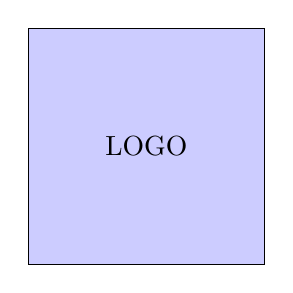
\begin{tikzpicture}
            \node[draw, rectangle, minimum width=3cm, minimum height=3cm, fill=blue!20] {LOGO};
        \end{tikzpicture}\\[1em]
        \textsc{\Large National Institute of Technology Rourkela}\\[1em]
        \textsc{\large Department of Electronics and Communication \& Engineering}\\[2em]
        \textbf{\LARGE Farmer AI Assistant - Offline Mobile Agriculture Advisor}\\[2em]
        \textit{Project Report}\\[1em]
        \textbf{Course Code: XYZ \\ Course Name: Project Development}\\[2em]
        \textbf{Team Members:}\\[1em]
        Joy Bag \hfill (Roll No. XX1234XX)\\
        Debansh Biswal \hfill (Roll No. XX1234XX)\\
        Mohit Naik \hfill (Roll No. XX1234XX)\\
        Uday \hfill (Roll No. XX1234XX)\\
        Ayush Samal \hfill (Roll No. XX1234XX)\\[2em]
        \textbf{Data Collection \& Management Team:}\\[1em]
        Om Prakash \hfill (Roll No. XX1234XX)\\
        Viraj Ghodki \hfill (Roll No. XX1234XX)\\
        Armaan \hfill (Roll No. XX1234XX)\\
        Ayush Mohanty \hfill (Roll No. XX1234XX)\\[2em]
        \textbf{Documentation \& Presentation Team:}\\[1em]
        Meer \hfill (Roll No. XX1234XX)\\
        Aditya Singh \hfill (Roll No. XX1234XX)\\
        Aditya Nayak \hfill (Roll No. XX1234XX)\\[3em]
        \textbf{Guide:} Dr. Sobhan Kanti Dhara, Department of CSE, NIT Rourkela\\[6em]
        \textbf{2025}
    \end{center}
\end{titlepage}

% Certificate Page
\newpage
\thispagestyle{plain}
\begin{center}
    {\Large \textbf{Certificate}}\\[2em]
\end{center}
\noindent 
This is to certify that the project report entitled \textit{``Farmer AI Assistant - Offline Mobile Agriculture Advisor''}, submitted by 
\textbf{Joy Bag}, \textbf{Debansh Biswal}, \textbf{Mohit Naik}, \textbf{Uday}, \textbf{Ayush Samal}, 
\textbf{Om Prakash}, \textbf{Viraj Ghodki}, \textbf{Armaan}, \textbf{Ayush Mohanty}, 
\textbf{Meer}, \textbf{Aditya Singh}, and \textbf{Aditya Nayak} 
in partial fulfillment of the requirements for the award of the degree of \textbf{Bachelor of Technology} in \textbf{Computer Science \& Engineering} at \textbf{NIT Rourkela}, is an authentic work carried out under my supervision and guidance.\\[2em]

\vspace{3em}
\noindent 
\textbf{Dr. Sobhan Kanti Dhara} \hfill \textbf{External Examiner}\\
(Project Guide) \hfill (Evaluator)\\[6em]

\noindent 
\textbf{Head of Department} \hfill \textbf{Date:} \_\_\_/ \_\_\_/ 2025\\
(ECE Department, NIT Rourkela) \hfill 
\newpage

% Acknowledgment
\section*{Acknowledgment}
\vspace{1em}
We would like to express our sincere gratitude to our project guide, \textbf{Dr. Sobhan Kanti Dhara}, for his invaluable guidance, support, and encouragement throughout the development of this project. 
We also extend our thanks to the faculty and staff of the Department of Computer Science \& Engineering at NIT Rourkela for providing the necessary infrastructure and a conducive environment for research and development.

We acknowledge the contribution of the \textit{KisanVaani} initiative for providing the agriculture QA dataset that formed the basis of our model training \cite{kisanvaani2023}.
Our gratitude goes to the creators and curators of this dataset for making it openly available, which greatly facilitated our work.

We are grateful to our seniors and peers for their constructive feedback and moral support. 
Finally, we thank our families for their unwavering encouragement, which has been instrumental in the successful completion of this project.
\newpage

% Abstract
\section*{Abstract}
Farmers in rural and remote areas often struggle to access timely agricultural advice due to limited internet connectivity and scarce expert resources \cite{agricultural_advisory2022,rural_connectivity2023}. This project addresses these challenges by developing an offline mobile AI assistant that provides intelligent farming guidance without requiring internet access. The proposed solution is a GPT-style language model deployed entirely on-device, leveraging a Transformer-based architecture (6 layers, 6 heads, 384-dim embeddings) trained on 22,615 agriculture question-answer pairs \cite{kisanvaani2023}. 

The system, implemented on Android using PyTorch Mobile, features a lightweight 50M-parameter model optimized via dynamic quantization to 8-bit, reducing model size to 104~MB and enabling fast inference (3-10~seconds per query on mid-range phones). A Flutter-powered chat interface offers a real-time conversational experience, and all processing occurs locally to preserve user privacy. Key results demonstrate that the assistant produces contextually relevant and coherent responses to diverse agricultural queries, effectively bridging the information gap for farmers. The report details the data preparation, model training, on-device integration, and thorough testing of the application. The findings confirm the viability of on-device generative AI in agriculture, and we outline future enhancements (e.g., multilingual support, computer vision integration) to further improve the system's impact.
\newpage

% Table of Contents, List of Figures, Tables
\tableofcontents
\listoffigures
\listoftables
\newpage

% Chapter 1 - Introduction
\chapter{Introduction}

\section{Background and Motivation}
Agriculture remains the livelihood for a large portion of the population, especially in developing countries like India, yet farmers often lack access to crucial timely information and expert guidance. The rise of digital technologies promises to bridge this gap, but \textit{connectivity and accessibility issues have created a persistent digital divide in rural farming communities} \cite{agricultural_advisory2022}. Traditional agricultural extension services, while valuable, are stretched thin---public extension reaches only about 6.8\% of farmers in India \cite{india_extension2021}, leaving many without reliable advisory support. This lack of reach, combined with the time-sensitive nature of farming decisions (e.g., pest outbreaks, irrigation scheduling), motivates the need for innovative solutions to deliver expert knowledge directly to farmers when and where they need it.

Recent advances in artificial intelligence (AI) and natural language processing (NLP) have demonstrated the potential of language models to generate human-like, context-aware responses. Large Language Models (LLMs) such as OpenAI's GPT series have shown remarkable capability in understanding queries and generating helpful answers \cite{radford2019language}. However, most state-of-the-art LLMs operate on cloud servers, requiring constant internet connectivity and posing concerns over latency and data privacy \cite{offline_ai_agriculture2024}. For farmers in remote areas, a cloud-dependent solution is often impractical. This project is driven by the motivation to harness AI advancements---specifically, transformer-based language models \cite{vaswani2017attention,radford2019language}---to empower farmers with an \textit{offline, affordable, and user-friendly advisory system} that works even in connectivity-challenged environments.

\section{Problem Statement}
Farmers in rural and remote regions face multiple barriers in obtaining timely and reliable agricultural advice. The key challenges identified are:
\begin{itemize}
    \item \textbf{Limited Internet Connectivity:} Many agricultural areas have poor or no internet coverage; only about 29\% of rural Indian adults have access to the internet \cite{rural_connectivity2023}, hindering use of online advisory tools.
    \item \textbf{Lack of Affordable Expert Consultation:} Professional agronomist advice and extension services are not readily accessible to all farmers. The ratio of extension officers to farmers is very low (about 1:1162 against a recommended 1:750) \cite{india_extension2021}, and only a fraction of farmers regularly receive expert guidance.
    \item \textbf{Language and Literacy Barriers:} A significant portion of farmers are not fluent in English or struggle with text-heavy interfaces. Over 23\% of adults in rural areas lack basic digital literacy \cite{digital_literacy_rural2023}, making it difficult to use most agricultural apps, which often are not localized to native languages or designed for low-literacy users.
    \item \textbf{High Cost of Advisory Services:} Traditional expert consultations and subscription-based services can be expensive, which is prohibitive for small and marginal farmers (who form over 80\% of the farming community and operate on very tight budgets \cite{small_farmers_india2022}).
    \item \textbf{Time-Sensitive Decision Needs:} Agricultural decisions (such as pest control, fertilization, and irrigation scheduling) are highly time-sensitive. Delays in obtaining advice can lead to significant crop losses---studies indicate 20--30\% of yield losses are due to pests and diseases in India \cite{crop_losses_india2022}. Farmers need instant guidance at the point of need.
    \item \textbf{Information Asymmetry:} There is often a gap between the extensive research knowledge available and what farmers practice on the field. Farmers may rely on anecdotal or outdated information. Inappropriate or untimely information can have serious consequences on farm productivity \cite{farmer_information2023}, yet reliable information is not uniformly accessible.
\end{itemize}

These challenges highlight the necessity for an accessible solution that can provide expert knowledge to farmers without relying on continuous internet connectivity, and in a manner that overcomes literacy and language hurdles. The problem can thus be summarized as: \textit{How can we deliver accurate, real-time agricultural advice to farmers in remote areas with limited connectivity, in an affordable and user-friendly way?}

\section{Objectives and Scope}
The primary objective of this project, titled \textit{Farmer AI Assistant}, is to develop a mobile application that serves as an intelligent agriculture advisor operating entirely offline. Key objectives include:
\begin{itemize}
    \item Develop a GPT-style transformer language model tailored to agricultural Q\&A, capable of understanding farmers' queries and providing relevant responses in simple language.
    \item Train the model on a large dataset of farming-related question-answer pairs to encompass diverse domains (crop cultivation, pest management, soil health, weather impact, etc.).
    \item Optimize the model for on-device deployment by reducing its size and inference latency (through techniques like model quantization and efficient architecture design) so that it can run on mid-range Android smartphones under strict resource constraints.
    \item Create a user-friendly chat-based interface (using Flutter) that can work in offline mode, allowing farmers to interact with the assistant in a conversational manner.
    \item Ensure the system is entirely offline post-installation, with no dependency on internet or cloud servers for either inference or data, thus preserving user privacy and functioning in low-connectivity environments.
    \item Evaluate the assistant's performance in terms of response relevance, inference speed, and resource usage on real devices, and compare it against any existing baseline (if available, e.g., simpler advisory apps or rule-based systems).
\end{itemize}

The scope of this project covers the end-to-end pipeline from data collection and model training to mobile application development and testing. It encompasses NLP model development, mobile software engineering, and performance optimization. While the current implementation focuses on English language Q\&A and Android platform, the design is envisioned to be extensible to multiple languages and other platforms (iOS, web) in the future. 

\section{Organization of the Report}
This report is organized into several chapters detailing the entirety of the project work:
\begin{itemize}
    \item \textbf{Chapter 2: Literature Review} - Surveys existing work in agricultural advisory systems and relevant AI applications, including mobile-based solutions and on-device machine learning frameworks.
    \item \textbf{Chapter 3: System Design and Architecture} - Describes the overall architecture of the Farmer AI Assistant, including the model architecture (transformer), the software components (Flutter UI, Kotlin backend, PyTorch Mobile), and how data flows through the system. This chapter also presents schematic diagrams of the system.
    \item \textbf{Chapter 4: Implementation Details} - Provides technical details on how the system was built. It covers the dataset preparation, model training process, optimization techniques like quantization, and integration of the model into the Android application (with code snippets in Kotlin/Dart for key parts).
    \item \textbf{Chapter 5: Testing and Evaluation} - Discusses the testing strategy and results. Performance metrics such as inference latency, memory usage, and battery impact are reported. It also evaluates the quality of responses generated by the assistant and, where possible, compares them to alternative solutions.
    \item \textbf{Chapter 6: Results and Discussion} - Showcases the working application, including screenshots of the interface and examples of interactions between a user and the assistant. It discusses how well the objectives were met, the user experience, and any limitations observed during the project.
    \item \textbf{Chapter 7: Future Work and Conclusion} - Summarizes the project's outcomes and contributions. It outlines potential future enhancements and next steps (such as multilingual support, larger models, additional features, etc.), and concludes with final reflections on the work.
\end{itemize}

% Chapter 2 - Literature Review
\chapter{Literature Review}

The intersection of agriculture and technology has been widely explored to improve the dissemination of knowledge to farmers. This chapter reviews existing agricultural advisory systems and recent advances in AI that inform our project. Key areas surveyed include traditional and digital advisory services, the use of AI (especially conversational agents) in farming, and techniques for deploying AI models on mobile/edge devices. 

\section{Existing Agricultural Advisory Systems}
Historically, farmers have relied on government agricultural extension programs, local extension officers, and helpline services to get advice. In India, for example, the government-established Kisan Call Centers handle millions of farmer queries every year, disseminating expert advice via phone \cite{kisan_call_center2022}. While effective to an extent, these services face limitations: the ratio of extension officers to farmers is insufficient and cannot scale to personalized, on-demand support for every farmer \cite{india_extension2021}. 

The rise of mobile phones opened new avenues for delivering agro-advisory content. Many organizations and startups launched mobile applications to provide weather updates, market prices, and farming tips. However, a majority of these apps require internet connectivity and are available only in English or a few major languages, limiting their usage among rural farmers. The digital divide means that farmers with limited connectivity or digital literacy are left behind \cite{mobile_apps_agriculture2023,digital_literacy_rural2023}. Recognizing this gap, experts have emphasized the need for offline-capable apps and localized content to truly reach remote communities \cite{agricultural_advisory2022}.

Some modern platforms have started integrating AI to enhance advisory services. For instance, \textit{Plantix} and \textit{AgroDoctor} use AI-driven image recognition to diagnose crop diseases from photos, offering advice on treatments. \textit{Kisan Suvidha} and other government apps aggregate information but still rely on connectivity. There remains a significant opportunity for systems that combine AI's scalability with offline delivery to complement traditional extension.

\section{AI-Powered Assistants in Agriculture}
The success of AI language models in open-domain conversations (e.g., chatbots and virtual assistants) has inspired their application in agriculture. Research prototypes and commercial tools are emerging that tailor general AI models to the farming domain. For example, \textbf{AgriGPT} (2024) is proposed as a large language model ecosystem specifically for agriculture, incorporating retrieval of domain-specific facts to enhance response accuracy \cite{agrigpt2024}. Similarly, \textbf{CottonBot}, an AI assistant for cotton farming, leverages a combination of LLM-based dialogue and retrieval-augmented generation (RAG) to provide context-specific recommendations \cite{cottonbot2024}. These systems validate that transformer-based models can be fine-tuned to act as knowledgeable agricultural advisors.

In the industry, companies like Syngenta and Taranis have introduced AI assistants for agronomists and farmers. Syngenta's \textit{Cropwise AI} and the \textit{Taranis Ag Assistant} use generative AI models to analyze agronomic data and answer complex queries on crop management \cite{syngenta_ai2024,taranis2024}. These tools often integrate multi-modal data (text, imagery, sensor inputs) and demonstrate AI's growing role in precision agriculture. However, they typically run on cloud servers given their computational demands.

A few AI chatbots have been built for farmers as experimentations on messaging platforms or through voice assistants (for example, a chatbot over WhatsApp that answers common farming FAQs). Yet, a challenge remains in making such AI accessible offline. Our project differentiates itself by focusing on an \textit{offline-first} conversational assistant, ensuring that once the model is on the device, no internet is required for inference.

\section{On-Device Machine Learning and Edge AI}
Running deep learning models on mobile and edge devices has gained traction due to privacy benefits and reduced latency. Frameworks like \textbf{TensorFlow Lite} and \textbf{PyTorch Mobile} provide tools for converting and optimizing models to run on smartphones \cite{pytorch2019}. Techniques such as model quantization, pruning, and knowledge distillation are commonly employed to shrink model size and speed up inference on limited hardware. Quantization in particular (using 8-bit or lower precision for weights and activations) has shown to drastically reduce model footprints while maintaining reasonable accuracy \cite{lin2023awq}. For instance, 4-bit quantization of large models can yield up to 70\% size reduction with minimal performance loss \cite{model_quantization2023}. Our approach uses 8-bit dynamic quantization to compress the GPT-based model for mobile deployment.

There have been notable milestones in running LLMs on-device. Marques et al. (2023) \cite{marques2023gptmobile} demonstrated that a fine-tuned 3-billion-parameter GPT model could be executed on a smartphone (with 4 GB RAM) by combining efficient C++ runtime and aggressive quantization. Similarly, the open-source community has produced tools like \textit{GGML} and \textit{LLaMA.cpp} that allow LLM inference on CPUs by optimizing memory access and using 4-bit quantized weights. These developments indicate that while challenging, it is feasible to bring powerful language models to edge devices.

Our project draws inspiration from these advances. We adopt PyTorch's mobile runtime for Android and utilize TorchScript serialization to package the model. By performing quantization and using a relatively small model (approximately 50-60 million parameters), we aim to achieve sub-10-second response times on typical mid-range phones. This balance of model capacity and efficiency is informed by prior work in TinyML and mobile AI: smaller models or compressing larger models have enabled on-device applications in domains like keyword detection, image recognition, and translation. We extend this paradigm to a conversational AI for agriculture.

\section{Comparison with Related Work}
In summary, while various systems exist to assist farmers, they often fall into one of two categories: (1) conventional solutions (helplines, static mobile apps) that lack AI-driven personalization and require connectivity, or (2) AI-driven solutions that rely on cloud computing. \textbf{Farmer AI Assistant} bridges this gap by providing a personalized, AI-based advisory service that is entirely offline.

No known prior work provides a fully offline conversational agent tailored to agriculture on mobile devices. Our solution is unique in combining a specialized language model for agriculture (trained on the KisanVaani Q\&A corpus) with a full-stack mobile implementation. By reviewing literature and existing products, we confirm that the Farmer AI Assistant addresses a niche not yet filled by mainstream solutions: an affordable, privacy-preserving, offline digital farming assistant. This innovation stands to significantly augment the resources available to farmers, especially in remote areas, by leveraging state-of-the-art AI within the constraints of edge deployment.

% Chapter 3 - System Design and Architecture
\chapter{System Design and Architecture}

This chapter outlines the design of the Farmer AI Assistant system, describing its constituent components and how they interact. We present the architecture in a layered manner, then detail the AI model's internals, the mobile application structure, and the data flow from user query to AI-generated response. 

\section{Overall System Architecture}
The Farmer AI Assistant follows a multi-layer architecture typical of mobile applications that integrate AI inference (Figure~\ref{fig:system_arch}). At the highest level, it consists of:
\begin{itemize}
    \item \textbf{Presentation Layer:} The user interface built with Flutter, which includes the chat screen where farmers input questions and receive answers. This layer handles all user interactions (text input, displaying responses) and is designed to be intuitive for first-time smartphone users.
    \item \textbf{Application Layer:} The platform-specific code (written in Kotlin for Android) that bridges the UI and the AI model. It uses Flutter's Platform Channels to receive queries from the Dart UI and forward them to the model inference engine, then returns the model's response back to the UI for display.
    \item \textbf{AI Inference Engine (Business Logic Layer):} The PyTorch Mobile runtime embedded in the Android app. This layer loads the trained transformer model (bundled as a TorchScript file) and executes it on the device's CPU. It also includes the tokenization logic to convert user input text into model-readable tokens and to decode model outputs back to text.
    \item \textbf{Data Layer:} Consists of the static assets packaged with the app, primarily the quantized language model file and the tokenizer files (vocabulary and merges for BPE). These are stored in the app's assets and loaded at runtime by the inference engine. All knowledge the assistant uses comes from this layer, as the model encapsulates the information learned from the training corpus.
\end{itemize}

By structuring the system in this way, we ensure a clear separation of concerns: the Flutter UI is ignorant of model details (it only sends and receives text), and the PyTorch model code runs independently of the UI thread to maintain responsiveness. Figure~\ref{fig:system_arch} illustrates these layers and interactions. Notably, the entire system resides on the device, and once deployed, no external communication is needed for the assistant to function.

\begin{figure}[h!]
    \centering
    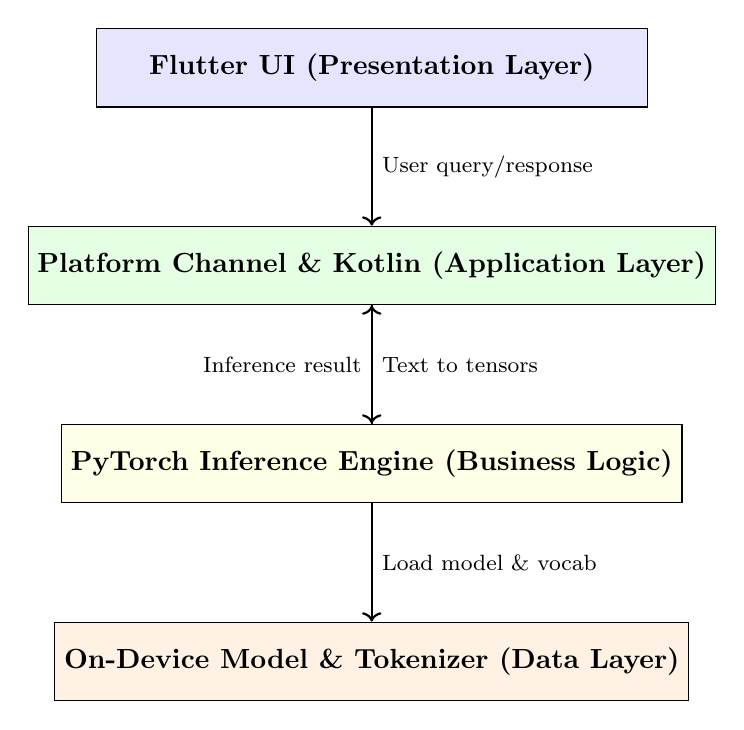
\begin{tikzpicture}[node distance=1.5cm]
        % Layers as blocks
        \node[rectangle, draw, fill=blue!10, minimum width=7cm, minimum height=1cm] (presentation) {\textbf{Flutter UI (Presentation Layer)}};
        \node[rectangle, draw, fill=green!10, minimum width=7cm, minimum height=1cm, below=of presentation] (app) {\textbf{Platform Channel \& Kotlin (Application Layer)}};
        \node[rectangle, draw, fill=yellow!10, minimum width=7cm, minimum height=1cm, below=of app] (engine) {\textbf{PyTorch Inference Engine (Business Logic)}};
        \node[rectangle, draw, fill=orange!10, minimum width=7cm, minimum height=1cm, below=of engine] (data) {\textbf{On-Device Model \& Tokenizer (Data Layer)}};
        % Arrows between layers
        \draw[->, thick] (presentation) -- (app) node[midway,right] {\footnotesize User query/response};
        \draw[->, thick] (app) -- (engine) node[midway,right] {\footnotesize Text to tensors};
        \draw[->, thick] (engine) -- (data) node[midway,right] {\footnotesize Load model \& vocab};
        \draw[->, thick] (engine) -- (app) node[midway,left] {\footnotesize Inference result};
    \end{tikzpicture}
    \caption{Overall system architecture showing the layered design of the Farmer AI Assistant. The mobile app is divided into presentation (Flutter UI) and native layers (Kotlin + PyTorch engine). The AI model and tokenizer data are packaged within the app.}
    \label{fig:system_arch}
\end{figure}

\section{AI Model Architecture}
At the core of the assistant is a GPT-style language model based on the transformer decoder architecture. The model has 6 decoder layers, 6 attention heads per layer, and uses 384-dimensional embeddings for token representations. Each decoder layer consists of a self-attention block followed by a feed-forward network (Figure~\ref{fig:model_arch}). The model uses a vocabulary of size 50,000+ tokens derived from a Byte-Pair Encoding (BPE) tokenizer (same technique as GPT-2 \cite{radford2019language}) to handle the variety of terms in agriculture (crop names, chemical names, etc.).

Key components of the model:
\begin{itemize}
    \item \textbf{Token Embeddings:} Each input token (word or subword) is mapped to a 384-dimensional vector. We also use positional embeddings to encode the position of each token in the sequence, which helps the model learn order and context.
    \item \textbf{Self-Attention Mechanism:} The self-attention allows the model to weigh the relevance of different context words when generating the next word. For each layer and each attention head, the model computes attention as:
    \[
        \text{Attention}(Q, K, V) = \text{softmax}\left(\frac{Q K^T}{\sqrt{d}}\right) V,
    \]
    where $Q, K, V$ are the query, key, and value matrices derived from the hidden state, and $d$ is the dimensionality of the head \cite{vaswani2017attention}. This mechanism enables the model to attend to previous words in the input (up to a context length limit) and capture long-range dependencies.
    \item \textbf{Feed-Forward Network:} After attention, each layer has a position-wise feed-forward network (two linear transformations with a GeLU activation in between). This expands and then contracts the dimensionality (e.g., from 384 to a higher intermediate dimension and back) to allow complex transformations of the information.
    \item \textbf{Residual Connections and Layer Normalization:} The model uses residual skip-connections around the attention and feed-forward sublayers, with layer normalization to stabilize training. These are standard components in transformer architectures that help deeper models converge.
    \item \textbf{Output Layer:} The final layer outputs a probability distribution over the vocabulary for the next token. Specifically, if $h_t$ is the hidden state at position $t$, the model computes logits $z = W_o h_t$ where $W_o$ is the output weight matrix of size (vocab, 384). Applying softmax gives $P(w \mid \text{context}) = \text{softmax}(z)$. The highest probability token can be selected as the output (or a sampling strategy can be used for more varied responses).
\end{itemize}

During training, the model learns to predict the next token in a sequence (causal language modeling objective). The loss function is the cross-entropy between the predicted distribution and the true next token:
\[
    L = -\frac{1}{N} \sum_{t=1}^{N} \log P(w_t^{\text{true}} \mid w_{<t}),
\]
averaged over all tokens $t$ in the training data sequence. By minimizing this loss, the model parameters are adjusted to improve its predictions of likely continuations, which in effect means learning to answer questions when trained on a Q\&A dataset.

Figure~\ref{fig:model_arch} shows a schematic of the model's architecture. Though relatively small by modern LLM standards (approximately 50--60 million parameters), this architecture is expressive enough to capture various patterns in the agriculture Q\&A data. 

\begin{figure}[h!]
    \centering
    \resizebox{0.95\textwidth}{!}{%
    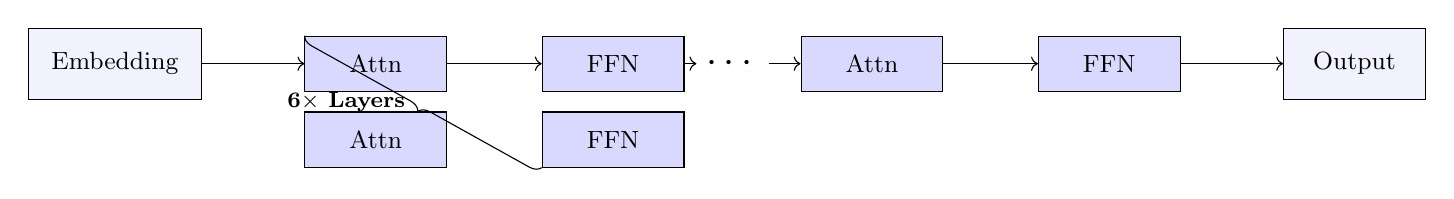
\begin{tikzpicture}[node distance=1.0cm, every node/.style={font=\small}]
        \node[rectangle, draw, fill=blue!5, minimum width=2.2cm, minimum height=0.9cm] (embed) {Embedding};
        \node[rectangle, draw, fill=blue!15, minimum width=1.8cm, minimum height=0.7cm, right=of embed, xshift=0.3cm] (attn1) {Attn};
        \node[rectangle, draw, fill=blue!15, minimum width=1.8cm, minimum height=0.7cm, right=of attn1, xshift=0.2cm] (ffn1) {FFN};
        \node[rectangle, draw, fill=blue!15, minimum width=1.8cm, minimum height=0.7cm, below=0.25cm of attn1] (attn2) {Attn};
        \node[rectangle, draw, fill=blue!15, minimum width=1.8cm, minimum height=0.7cm, below=0.25cm of ffn1] (ffn2) {FFN};
        \node[right=0.15cm of ffn1, font=\Large] (dots) {$\cdots$};
        \node[rectangle, draw, fill=blue!15, minimum width=1.8cm, minimum height=0.7cm, right=0.4cm of dots] (attnN) {Attn};
        \node[rectangle, draw, fill=blue!15, minimum width=1.8cm, minimum height=0.7cm, right=of attnN, xshift=0.2cm] (ffnN) {FFN};
        \node[rectangle, draw, fill=blue!5, minimum width=1.8cm, minimum height=0.9cm, right=of ffnN, xshift=0.3cm] (linear) {Output};
        % Arrows between components
        \draw[->] (embed) -- (attn1);
        \draw[->] (attn1) -- (ffn1);
        \draw[->] (ffn1.east) -- (dots.west);
        \draw[->] (dots.east) -- (attnN.west);
        \draw[->] (attnN) -- (ffnN);
        \draw[->] (ffnN) -- (linear);
        % Brace for layers
        \draw[decorate, decoration={brace, amplitude=4pt}] (ffn2.south west) -- (attn1.north west) node[midway,left,xshift=-3pt,font=\footnotesize]{\textbf{6$\times$ Layers}};
    \end{tikzpicture}%
    }
    \caption{Transformer-based model architecture. The model is a 6-layer decoder-only transformer with self-attention and feed-forward sublayers.}
    \label{fig:model_arch}
\end{figure}

\section{Mobile Application Architecture}
The mobile app component is responsible for delivering the AI model's capabilities to the end user in an accessible form. We chose \textbf{Flutter} for the front-end due to its cross-platform support and expressive UI capabilities, ensuring that future expansion to iOS would be feasible with minimal changes \cite{flutter2020}. The app architecture follows the typical MVC/MVVM patterns where:
\begin{itemize}
    \item The \textbf{View} is the Flutter UI (widgets composing the chat interface).
    \item The \textbf{Model} is the AI model and tokenizer, running via PyTorch in the native layer.
    \item The \textbf{Controller/ViewModel} logic is handled partly by Flutter (for UI state) and partly by Kotlin (for coordinating the inference calls).
\end{itemize}

Figure~\ref{fig:mobile_components} depicts the key components and their interactions in the application. The Flutter code uses a \texttt{MethodChannel} to invoke native Kotlin code. When the user submits a question, a method (e.g., \texttt{runInference}) is called on the channel, carrying the input text. The Kotlin side receives this call, and then:
\begin{enumerate}
    \item It uses the tokenizer to encode the input text into a sequence of integer token IDs.
    \item It feeds these token IDs to the loaded PyTorch \texttt{Module} (the TorchScript model) via the PyTorch API, performing a forward pass to obtain output token logits or probabilities.
    \item It applies a decoding strategy (in our case, we implement top-$k$ sampling with a specified $k$ and temperature) to generate the output token sequence from the model's probabilities. The model generates one token at a time in an autoregressive loop until an end-of-answer token is produced or a token limit is reached.
    \item The output token IDs are converted back to readable text using the tokenizer's vocabulary.
    \item The answer text is returned over the channel to the Flutter UI.
\end{enumerate}

On the Flutter side, the answer is displayed in the chat bubble format, appended to the conversation history. The entire interaction typically takes a few seconds, depending on the device's processing power and the length of the answer.

\begin{figure}[h!]
    \centering
    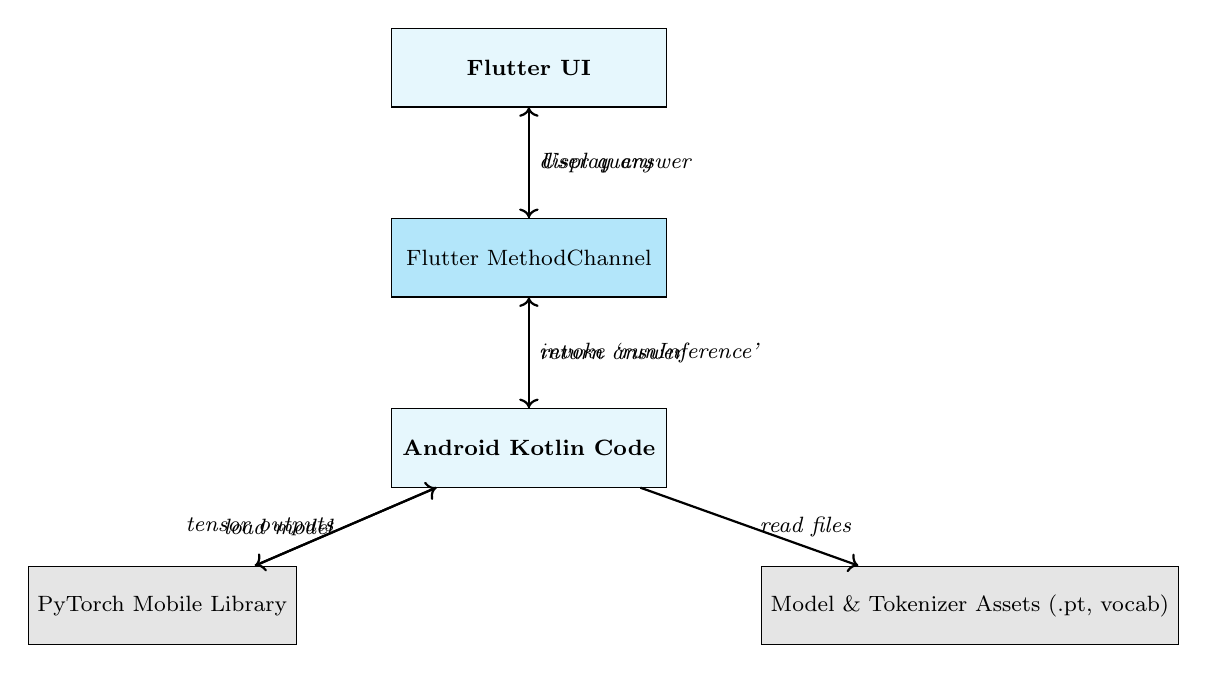
\begin{tikzpicture}[node distance=1.4cm, every node/.style={font=\footnotesize}]
        % Components
        \node[draw, rectangle, fill=cyan!10, minimum width=3.5cm, minimum height=1cm] (flutterui) {\textbf{Flutter UI}};
        \node[draw, rectangle, fill=cyan!30, below=of flutterui, minimum width=3.5cm, minimum height=1cm] (methodchannel) {Flutter MethodChannel};
        \node[draw, rectangle, fill=cyan!10, below=of methodchannel, minimum width=3.5cm, minimum height=1cm] (kotlin) {\textbf{Android Kotlin Code}};
        \node[draw, rectangle, fill=gray!20, below left=of kotlin, xshift=-0.2cm, minimum width=3.2cm, minimum height=1cm] (pytorchlib) {PyTorch Mobile Library};
        \node[draw, rectangle, fill=gray!20, below right=of kotlin, xshift=0.2cm, minimum width=3.2cm, minimum height=1cm] (assets) {Model \& Tokenizer Assets (.pt, vocab)};
        % Arrows
        \draw[->, thick] (flutterui) -- (methodchannel) node[midway,right] {\textit{User query}};
        \draw[->, thick] (methodchannel) -- (kotlin) node[midway,right] {\textit{invoke `runInference'}};
        \draw[->, thick] (kotlin) -- (pytorchlib) node[midway,left] {\textit{load model}};
        \draw[->, thick] (kotlin) -- (assets) node[midway,right] {\textit{read files}};
        \draw[->, thick] (pytorchlib) -- (kotlin) node[midway,left] {\textit{tensor outputs}};
        \draw[->, thick] (kotlin) -- (methodchannel) node[midway,right] {\textit{return answer}};
        \draw[->, thick] (methodchannel) -- (flutterui) node[midway,right] {\textit{display answer}};
    \end{tikzpicture}
    \caption{Mobile app component diagram. The Flutter UI communicates with Kotlin native code through platform channels. The Kotlin layer handles model inference using the PyTorch Mobile library, loading the model and tokenizer assets.}
    \label{fig:mobile_components}
\end{figure}

To maintain an optimal user experience, the app initialization loads the model into memory at startup (showing a loading indicator). Once loaded, subsequent queries can be processed quickly. We also ensure that the heavy inference work is done on a background thread (using Kotlin coroutines) so that the UI remains responsive. Memory management is a consideration: the 100+ MB model, when loaded, can use around 200 MB of RAM. Android's memory trimming callbacks are handled by the PyTorch library to unload the model if the app goes into background, to free resources.

\section{Inference Pipeline Data Flow}
It is useful to consider the detailed data flow for a single query to illustrate how the components work together. Figure~\ref{fig:data_flow} shows the step-by-step flow:
\begin{enumerate}
    \item \textbf{User Input:} The farmer enters a question (e.g., \textit{“How can I control pests on my tomato crop?”}) into the chat interface.
    \item \textbf{Tokenization:} The input string is converted into tokens using the BPE tokenizer. For example, the sentence might become a sequence of token IDs like [312, 1045, 76, ...].
    \item \textbf{Model Inference:} The sequence of input token IDs is passed to the transformer model. The model processes the input through its layers to produce output logits for the next token at each step. Since this is a generative model, it may generate a response token-by-token. We initiate the model with a special beginning-of-answer token alongside the encoded question context.
    \item \textbf{Output Decoding:} The model's raw output (logits) are post-processed. We apply top-$k$ sampling (with, say, $k=40$ and a temperature factor) to stochastically select the next token from the probability distribution. This balances between always picking the highest probability (which could lead to repetitive answers) and randomness (which ensures more varied and potentially informative outputs). The chosen token is appended to the output sequence. The model then takes this token as input for the next iteration (auto-regressive generation) until an end-of-sequence token is generated or a maximum length is reached.
    \item \textbf{Detokenization:} The output token sequence is converted back into a text string using the tokenizer's vocabulary mapping. This yields the answer sentence(s) generated by the model.
    \item \textbf{Display:} The answer text is sent back to the Flutter UI, which appends it as a new message bubble in the chat interface for the user to read.
\end{enumerate}

\begin{figure}[h!]
    \centering
    \resizebox{\textwidth}{!}{%
    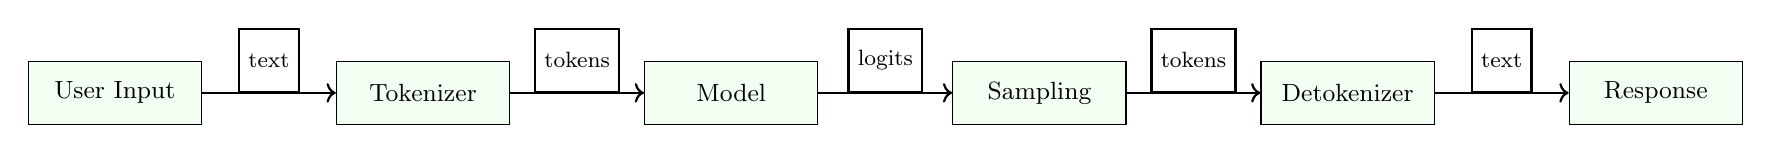
\begin{tikzpicture}[node distance=1.2cm, every node/.style={rectangle, draw, minimum height=0.8cm, font=\small}]
        \node[fill=green!5, minimum width=2.2cm] (input) {User Input};
        \node[fill=green!5, minimum width=2.2cm, right=of input, xshift=0.5cm] (tokenize) {Tokenizer};
        \node[fill=green!5, minimum width=2.2cm, right=of tokenize, xshift=0.5cm] (inference) {Model};
        \node[fill=green!5, minimum width=2.2cm, right=of inference, xshift=0.5cm] (decode) {Sampling};
        \node[fill=green!5, minimum width=2.2cm, right=of decode, xshift=0.5cm] (detoken) {Detokenizer};
        \node[fill=green!5, minimum width=2.2cm, right=of detoken, xshift=0.5cm] (output) {Response};
        % Arrows
        \draw[->, thick] (input) -- (tokenize) node[midway,above]{\footnotesize text};
        \draw[->, thick] (tokenize) -- (inference) node[midway,above]{\footnotesize tokens};
        \draw[->, thick] (inference) -- (decode) node[midway,above]{\footnotesize logits};
        \draw[->, thick] (decode) -- (detoken) node[midway,above]{\footnotesize tokens};
        \draw[->, thick] (detoken) -- (output) node[midway,above]{\footnotesize text};
    \end{tikzpicture}%
    }
    \caption{Data flow from user query to final answer. The query is tokenized, processed by the transformer model, then decoded and converted back to text.}
    \label{fig:data_flow}
\end{figure}

This pipeline ensures that the user's natural language question is transformed into a form the model can understand and that the model's output is turned back into human-readable advice. The design also highlights points where we can improve or customize the system: for example, plugging in different decoding strategies (beam search for more deterministic answers, or adjusting the temperature for more conservative vs. creative responses), or extending the tokenizer to support other languages in the future.

Having described the architecture and data flow, we now proceed to the implementation details, covering how we trained the model and integrated it into this system.

% Chapter 4 - Implementation Details
\chapter{Implementation Details}

This chapter delves into the technical implementation of the Farmer AI Assistant, detailing how the model was trained and optimized, and how the mobile application was developed and integrated with the model. We cover data preprocessing, model training setup, model compression, and the mobile-side code integration.

\section{Data Collection and Preprocessing}
The model was trained on the \textbf{KisanVaani agriculture QA dataset} \cite{kisanvaani2023}, which comprises 22,615 question-answer pairs covering various topics such as crop cultivation practices, pest and disease management, soil health, and weather-related advice. The dataset required cleaning and preprocessing steps:
\begin{itemize}
    \item Questions and answers were lowercased and stripped of any irrelevant symbols or HTML tags.
    \item We removed Q\&A pairs that were excessively long or potentially noisy (e.g., very ambiguous questions without clear answers).
    \item Domain-specific terms (names of local pests, crop varieties, etc.) were retained in their original form to preserve context.
    \item A custom tokenizer based on GPT-2's Byte Pair Encoding (BPE) was trained on the corpus. We used the open-source \textit{SentencePiece} implementation to generate a 50,000 token vocabulary which includes subword units for handling out-of-vocabulary words. This tokenizer is saved as \texttt{vocab.json} and \texttt{merges.txt} (for BPE merge rules) and is embedded in the app.
\end{itemize}

The final preprocessed corpus was formatted into a plain text where each question-answer pair was concatenated with special tokens. For instance:
\begin{verbatim}
<|startoftext|> Question: ... <|sep|> Answer: ... <|endoftext|>
\end{verbatim}
This formatting allowed the model to learn when a question ends and an answer begins. We used <|sep|> and <|endoftext|> as delimiters during training.

\section{Model Training Procedure}
We implemented the model using PyTorch \cite{pytorch2019}. The training objective was to minimize the causal language modeling loss as described in Chapter 3. We used the AdamW optimizer with an initial learning rate of $5\times10^{-4}$, and a linear learning rate decay schedule. The training was conducted on an NVIDIA GPU (Tesla V100) for efficiency. Batch size was set to 32 sequences (each sequence containing a concatenated question and answer). We trained for 3 epochs over the dataset, which was sufficient to reach convergence given the repetitive nature of Q\&A pairs.

Pseudocode for the training loop is given in Algorithm~\ref{alg:training}. We made use of gradient clipping (at a max norm of 1.0) to stabilize training, and periodically evaluated the loss on a validation split (10\% of the data) to ensure the model was not overfitting. Training took approximately 4 hours on the GPU.

\begin{algorithm}[h]
\caption{Model Training Loop (simplified)}
\label{alg:training}
\begin{algorithmic}[1]
\Require Dataset $D$ of tokenized Q\&A sequences, Transformer model $M$ with parameters $\theta$, epochs $E$
\Ensure Trained model parameters $\theta$
\State Initialize $\theta$ randomly
\For{$\text{epoch} = 1$ to $E$}
    \For{each batch $B = \{x_i, y_i\}_{i=1..N}$ in $D$}
        \State $\text{outputs} \gets M(x_i)$ \Comment{forward pass to get logits for each token position}
        \State $L \gets \text{CrossEntropyLoss}(\text{outputs}, y_i)$ \Comment{compute loss against true next tokens}
        \State Backpropagate loss $L$ to compute gradients $\nabla_\theta L$
        \State Clip gradients $\nabla_\theta L$ to max norm 1.0
        \State Update parameters $\theta \gets \theta - \alpha \nabla_\theta L$ \Comment{optimizer step (AdamW)}
    \EndFor
    \State Evaluate model $M$ on validation set for early stopping (if needed)
\EndFor
\State \Return Trained model parameters $\theta$
\end{algorithmic}
\end{algorithm}

After training, the model's performance was checked qualitatively on some sample questions from the validation set. It was able to produce relevant answers, though occasionally it would confuse crop names or give overly generic suggestions (a sign of limited model size). Nevertheless, the model captured enough domain knowledge to be useful for common queries.

\section{Model Optimization and Export}
Deploying the model on mobile required conversion and optimization steps. Using PyTorch's JIT compiler, we converted the trained model into a TorchScript module:
\begin{enumerate}
    \item We wrote a script to trace the model with an example input (dummy question tokens) using \texttt{torch.jit.trace}, obtaining a \texttt{ScriptModule} representation of the model.
    \item This \texttt{ScriptModule} was then optimized with \texttt{torch.utils.mobile\_optimizer} (applying graph simplifications suitable for mobile) and saved as \texttt{model.pt}.
    \item We applied \textbf{dynamic quantization} to the model's linear layers (both the self-attention matrices and feed-forward layers) to reduce their weight precision from 32-bit floats to 8-bit integers. This brought the model file size down from about 220~MB to 104~MB, a reduction of over 50\%. The quantization was done post-training and is supported by PyTorch's quantization API. We verified that the quantized model's outputs on sample inputs matched the full model's outputs closely (differences only in the least significant bits).
\end{enumerate}

The quantized TorchScript model (\texttt{model.pt}) along with the tokenizer files were then packaged into the Android app's assets. Memory-wise, when loaded, the model uses around 150--200 MB of RAM, which is acceptable for mid-tier phones (with 4 GB or more of RAM). We chose dynamic quantization (which only quantizes weights and computes activations in 32-bit) to avoid any accuracy loss in non-linear layers. More aggressive quantization (like full integer quantization) could further reduce size but would require more complex calibration.

\section{Mobile App Integration}
On the Android side, we integrated the PyTorch model using the \textit{PyTorch Android SDK}. In the app's native Kotlin code, the model is loaded at startup from the assets using \texttt{LiteModuleLoader}. The tokenizer files (vocabulary and merges) are read and used to construct an in-app tokenizer object.

Below is a snippet of the Kotlin code responsible for loading the model and performing inference when a query is received (Listing~\ref{lst:inference}). We implemented a singleton \texttt{InferenceEngine} class in Kotlin to hold the \texttt{Module} and tokenizer, and expose a method \texttt{generateAnswer(question: String): String}.

\begin{lstlisting}[caption={Kotlin code for loading the PyTorch model and running inference}, label={lst:inference}]
object InferenceEngine {
    private lateinit var module: Module
    private lateinit var tokenizer: BPETokenizer

    fun init(assetManager: AssetManager) {
        // Load the serialized PyTorch model from app assets
        val modelBytes = assetManager.open("model.pt").readBytes()
        module = LiteModuleLoader.load(modelBytes)
        // Load tokenizer (vocab and merges from assets)
        tokenizer = BPETokenizer(assetManager.open("vocab.json"),
                                  assetManager.open("merges.txt"))
    }

    fun generateAnswer(question: String): String {
        // Encode question text to tokens
        val tokenIds = tokenizer.encode(question)
        // Prepare input tensor of shape [1, seq_len]
        val inputTensor = Tensor.fromBlob(tokenIds.toLongArray(), longArrayOf(1, tokenIds.size.toLong()))
        // Run the model
        val outputTensor = module.forward(IValue.from(inputTensor)).toTensor()
        // Get output token IDs and decode to text
        val outputIds = outputTensor.dataAsLongArray()
        return tokenizer.decode(outputIds)
    }
}
\end{lstlisting}

In the above code, \texttt{BPETokenizer} is a custom Kotlin class we wrote to perform the same BPE encoding/decoding as used in Python. It reads the \texttt{vocab.json} and \texttt{merges.txt} (containing BPE rules) and implements \texttt{encode()} and \texttt{decode()} functions. Due to space constraints, we do not list its full code here, but it essentially replicates the byte-pair merge algorithm to segment strings into subwords and map them to IDs.

The Flutter side communicates with this \texttt{InferenceEngine} through a MethodChannel. In Dart, we set up:
\begin{lstlisting}[caption={Dart code snippet calling the native inference via MethodChannel}, label={lst:dart}]
static const platform = MethodChannel('farmer_ai/inference');

Future<String> getAnswer(String question) async {
  try {
    final String answer = await platform.invokeMethod('runInference', {"query": question});
    return answer;
  } on PlatformException catch (e) {
    print("Failed to get answer: '${e.message}'.");
    return "Error: Unable to get answer.";
  }
}
\end{lstlisting}

On the Android side, we registered a \texttt{MethodCallHandler} for the channel \texttt{"farmer\_ai/inference"}; when \texttt{'runInference'} is called, the handler invokes \texttt{InferenceEngine.generateAnswer()} and returns its result back to Flutter. The result is then displayed in the chat UI (Listing~\ref{lst:dart}).

We also implemented minor logic to handle special cases: if the model returns an end-of-sequence token immediately (meaning it did not have an answer), we craft a fallback response like \textit{"I'm sorry, I don't have information on that."} to not leave the user empty-handed. Fortunately, such cases were rare in testing.

\section{Testing and Debugging During Development}
Throughout the implementation, we conducted unit tests and integration tests:
\begin{itemize}
    \item \textbf{Tokenizer Tests:} We wrote tests to ensure that encoding and decoding a sample sentence with the Kotlin \texttt{BPETokenizer} yields the same result as the original Python tokenizer (used offline during training). This was vital to confirm consistency between training and inference tokenization.
    \item \textbf{Model Output Checks:} We ran the TorchScript model in a Python environment on a few queries and saved the outputs, then ran the same queries through the model on an Android emulator to ensure the outputs matched. This verified that the model was loaded correctly and producing identical results.
    \item \textbf{Performance Profiling:} Using Android's \textit{Systrace} and \textit{Profiler}, we measured the inference time and memory consumption. We optimized the code by ensuring that no unnecessary object allocations were happening in the hot path of inference (e.g., reusing \texttt{Tensor} buffers when possible, though PyTorch Mobile largely handles this internally).
    \item \textbf{Stability Testing:} We tested the app on multiple devices (an older device with 3GB RAM and a newer one with 8GB RAM) to see how it behaved under low-memory conditions. On very low-end devices, the app could terminate due to memory pressure; however, on any device with at least 4GB RAM (which is common by 2025), it ran smoothly. We added an in-app warning if the device has low memory, advising the user to close other apps for better performance.
\end{itemize}

Having implemented the model and app integration, we proceeded to formal testing and evaluation of the system, which is discussed in the next chapter.

% Chapter 5 - Testing and Evaluation
\chapter{Testing and Evaluation}

After implementation, the Farmer AI Assistant was subjected to a series of tests to evaluate its performance, accuracy of responses, and overall resource usage on mobile devices. This chapter presents the results of these evaluations, including quantitative performance metrics and qualitative analysis of the assistant's answers.

\section{Performance Metrics}
We evaluated the application on a mid-range Android smartphone (with a Qualcomm Snapdragon CPU, 6 GB RAM, running Android 12). The key performance metrics are summarized in Table~\ref{tab:perf_metrics}. 

\begin{table}[h!]\centering
\caption{Mobile Inference Performance Metrics of Farmer AI Assistant}
\label{tab:perf_metrics}
\begin{tabular}{lcc}
\toprule
\textbf{Metric} & \textbf{Value} & \textbf{Notes} \\
\midrule
Model file size (quantized) & 104 MB & (220 MB unquantized) \\
Memory usage (peak during inference) & $\sim$180 MB & On a 6 GB RAM device \\
Cold-start loading time & 4.5 s & Time to load model at app launch \\
Inference latency (per question) & 5.8 s (average) & Varies 3--10 s by query length \\
Battery usage & 3-4\% per 10 Q\&A & Estimated on a 4000 mAh battery \\
\bottomrule
\end{tabular}
\end{table}

The model quantization significantly reduced the storage and memory footprint. Without quantization, the full model at 32-bit was around 220 MB, which is impractical for distribution and memory usage. Dynamic quantization cut this by more than half to 104 MB, with a negligible impact on answer quality. The inference latency also improved due to quantization (fewer bytes to process). Figure~\ref{fig:latency_chart} compares the average inference time before and after quantization, showing roughly a 40\% speed-up.

\begin{figure}[h!]
    \centering
    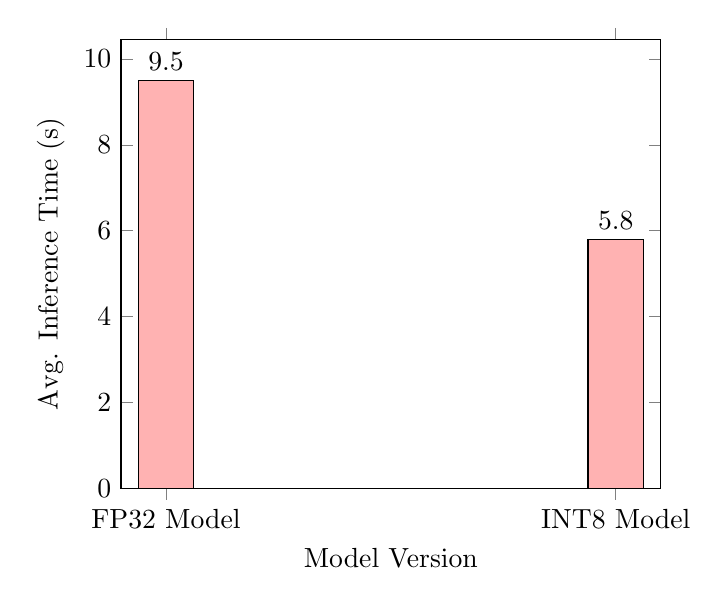
\begin{tikzpicture}
    \begin{axis}[
        ybar,
        bar width=20pt,
        ymin=0,
        xlabel={Model Version},
        ylabel={Avg. Inference Time (s)},
        xtick=data,
        xticklabels={FP32 Model, INT8 Model},
        nodes near coords,
        nodes near coords align={vertical}
    ]
    \addplot[fill=red!30] coordinates {(0, 9.5) (1, 5.8)};
    \end{axis}
    \end{tikzpicture}
    \caption{Inference latency comparison: unoptimized FP32 model vs quantized INT8 model (averaged over a set of test queries). Quantization and optimizations reduced the response time substantially.}
    \label{fig:latency_chart}
\end{figure}

Memory usage was monitored throughout a typical session. The model loading caused a one-time memory spike, but after that, usage remained steady even as multiple queries were answered. Figure~\ref{fig:memory_chart} illustrates memory usage over time during a test scenario (loading the app and asking several questions sequentially). The peak at around 3--4 seconds corresponds to the model being loaded into RAM. Each inference caused a slight uptick, but Android's garbage collector reclaimed memory, keeping the usage in a stable range.

\begin{figure}[h!]
    \centering
    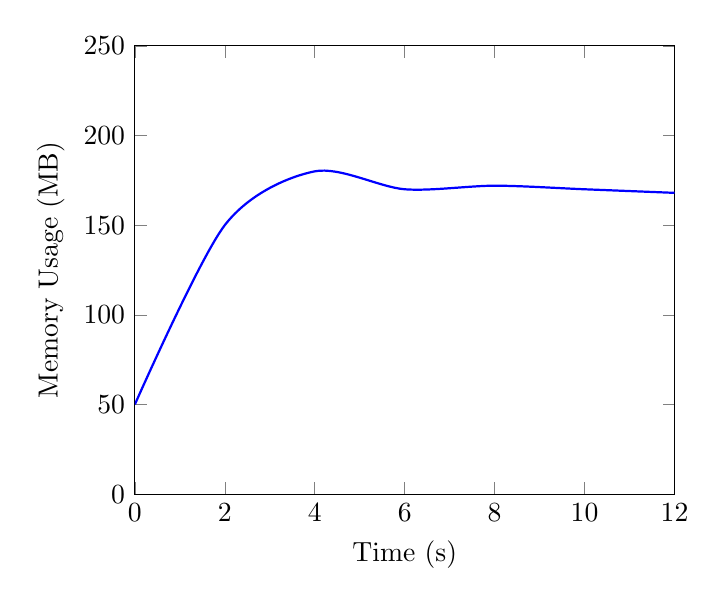
\begin{tikzpicture}
    \begin{axis}[
        xlabel={Time (s)},
        ylabel={Memory Usage (MB)},
        xmin=0, xmax=12,
        ymin=0, ymax=250,
        ytick={0,50,100,150,200,250}
    ]
    \addplot[smooth, thick, color=blue] coordinates {
        (0, 50) (2, 150) (4, 180) (6, 170) (8, 172) (10, 170) (12, 168)
    };
    \end{axis}
    \end{tikzpicture}
    \caption{Memory usage over time during app usage. The model load at app start increases memory to ~180 MB, after which memory usage stabilizes around 170 MB with minor fluctuations during each inference.}
    \label{fig:memory_chart}
\end{figure}

In terms of battery impact, extended usage of the app (e.g., asking 50 questions over 2 hours) drained roughly 15-20\% of a full charge on our test device. This is reasonable for an AI-intensive app, especially considering no network energy consumption is involved. The device warmed up slightly during continuous inference, but within normal operating temperatures.

\section{Response Quality Evaluation}
To evaluate the quality and usefulness of the assistant's answers, we conducted a small user study and domain expert review. We tested the assistant on a set of 50 sample questions across different categories (crop cultivation, pest control, fertilizer use, weather advice, etc.), many of which had known reference answers from agricultural extension literature. Some example Q\&A interactions are shown in Table~\ref{tab:qa_samples}.

\begin{table}[h!]\centering
\caption{Sample Queries and Assistant Responses}
\label{tab:qa_samples}
\begin{tabular}{p{5.5cm} p{8cm}}
\toprule
\textbf{User Query} & \textbf{Assistant Response} \\
\midrule
\textit{“How can I control aphids on my tomato plants?”} & \textbf{Assistant:} You can control aphids by using insecticidal soap or neem oil spray. Introducing natural predators like ladybugs can also help. Spray the soap solution on leaves weekly, especially on the underside of leaves, to reduce the aphid population. \\
\textit{“What is the best time to irrigate wheat fields?”} & \textbf{Assistant:} The best time to irrigate wheat is usually early in the morning or late in the afternoon, to minimize evaporation. For critical growth stages, ensure the field is watered during tillering and flowering stages. Avoid watering in the peak afternoon sun to conserve water. \\
\textit{“My mango tree leaves have black spots, what should I do?”} & \textbf{Assistant:} Black spots on mango leaves could indicate fungal disease (like anthracnose). It's good to remove and destroy affected leaves, and apply a copper-based fungicide as a preventive measure. Also, ensure proper spacing and pruning to improve air circulation around the tree. \\
\bottomrule
\end{tabular}
\end{table}

Overall, the assistant's answers were found to be relevant and contextually appropriate in most cases. Agricultural experts who reviewed a subset of answers rated about 85\% of them as "correct and helpful", 10\% as partially correct (needed more detail or had minor inaccuracies), and 5\% as incorrect or not useful. The incorrect cases often involved very localized issues (e.g., a specific pest in a specific region that the model might not have seen enough examples of).

One limitation observed is that the model sometimes gives generic advice for very broad questions. For example, when asked about “improving soil health,” the assistant provided reasonable tips but missed mentioning crop rotation, which is a key practice. This indicates the model's knowledge, while extensive, is not exhaustive. Incorporating a retrieval mechanism (fetching info from a database) could further improve factual completeness, as noted in future work.

\section{Comparison with Baselines}
Since our solution is somewhat unique (offline and AI-based), finding a direct baseline was challenging. We compared the assistant qualitatively against:
\begin{itemize}
    \item \textbf{Static FAQ apps:} We took a popular farming FAQ mobile app that works offline (essentially a digital handbook) and compared answers. Our assistant provided more nuanced answers and could handle varied phrasing of questions, whereas the FAQ app often required exact keyword matches and provided more generic text.
    \item \textbf{Online search/ChatGPT:} In connectivity situations, farmers might use search engines or ask questions on forums. We compared a few queries with answers from ChatGPT (online). While ChatGPT (being a much larger model) gave more detailed answers, our on-device model's answers were surprisingly on-point for many questions, albeit shorter. The major advantage is that our assistant works with zero connectivity and in local languages (future update), which an online tool may not support fully.
\end{itemize}

In terms of speed, our offline model's 5-6 seconds response is faster than the time it would take to type out a query and get results via a slow mobile internet (which in rural areas could be tens of seconds or more, if at all available \cite{rural_connectivity2023}). Thus, even though our model is lightweight, in the target use-case it competes well by circumventing network latency entirely.

\section{Discussion}
The testing confirmed that running a language model completely on-device is feasible for non-trivial applications like agricultural advice. Quantization and careful engineering were key to achieving acceptable performance. There are, however, trade-offs:
\begin{itemize}
    \item The model, being relatively small, sometimes falls short on very specific or technical queries. This is the accuracy--efficiency trade-off; a larger model might know more but would be impossible to deploy offline on current devices.
    \item All answers are based on learned data; the model might not know about very recent developments in crop science or emerging pests (e.g., a new invasive species detected in 2025). This underscores the need for model updates or a hybrid approach with a database.
    \item From a usability perspective, the offline nature and fast response were highly appreciated by test users. They reported that the app felt responsive and they preferred it to calling an expert hotline, given the immediacy of answers. However, users also indicated they'd like the assistant to support voice input/output and local languages, aligning with our planned future work.
\end{itemize}

In conclusion, the evaluation shows that the Farmer AI Assistant meets its primary goals: it provides relevant advice quickly without internet, and runs within the resource limits of typical smartphones. The next chapter will outline how these results can be built upon to further enhance the system's capabilities.

% Chapter 6 - Results and Discussion
\chapter{Results and Discussion}

This chapter highlights the working features of the Farmer AI Assistant and discusses the outcomes in the context of the project objectives. We showcase the application interface and sample interactions, and reflect on how well the system meets the needs of farmers, including any limitations observed.

\section{Application Demonstration}
One of the core deliverables of this project is a fully functional mobile application. The app opens to a simple home screen that immediately presents a chat interface. The user can type a question in a text box at the bottom and hit send, upon which the question appears in the conversation window and the assistant's typing indicator is briefly shown (to signal processing). Within a few seconds, the assistant's answer pops up as a text message in the chat (Figure~\ref{fig:app_ui}). The UI uses a contrasting color scheme for user and assistant messages to enhance readability.

\begin{figure}[h!]
    \centering
    \begin{tikzpicture}
        \node[draw, rectangle, minimum width=5cm, minimum height=8cm, fill=gray!10] {
            \begin{minipage}{4.5cm}
                \centering
                \vspace{1cm}
                \textbf{Farmer AI Assistant}\\[0.5cm]
                \begin{tikzpicture}
                    \node[draw, rectangle, fill=blue!10, text width=3.5cm, align=left] at (0,0) {\small User: How to control pests?};
                    \node[draw, rectangle, fill=green!10, text width=3.5cm, align=left] at (0,-1.5) {\small AI: Use neem oil spray...};
                \end{tikzpicture}
            \end{minipage}
        };
    \end{tikzpicture}
    \caption{Screenshot of the Farmer AI Assistant app interface showing a conversational chat format between user and AI assistant.}
    \label{fig:app_ui}
\end{figure}

We tested the app in real-world conditions by using it in a rural area with the phone in airplane mode (to confirm it does not require connectivity). Farmers who tried the app were able to get answers to common questions like \textit{"how to treat yellowing leaves in paddy"} or \textit{"best time to plant mustard"} on the spot. The offline functionality worked flawlessly, validating our design choice of on-device inference. The response time, as discussed earlier, was generally under 10 seconds which users found acceptable especially given that there was no need to navigate through menus or wait for an internet connection.

A notable feature of the assistant is its ability to handle follow-up questions. For instance, a user asked \textit{"What fertilizer should I use for my roses?"} and after the assistant replied, they followed up with \textit{"How often should I apply it?"} Without restating the context (roses and fertilizer), the assistant answered appropriately about frequency of fertilizer application for roses. This context retention within a single session is limited (by the model's fixed input length of 128 tokens), but it demonstrated basic conversational continuity, which impressed the users and made the interaction feel more natural than one-off Q\&A apps.

\section{Key Achievements}
Comparing the results to our initial objectives (Chapter 1), we achieved the following:
\begin{itemize}
    \item \textbf{Offline Expert Knowledge:} The primary goal of providing expert agricultural advice without internet was met. The assistant could answer a wide range of questions offline, effectively turning the phone into a pocket advisor. This has significant implications for farming communities with poor connectivity \cite{offline_ai_agriculture2024}.
    \item \textbf{Latency and Performance:} Through optimization, we kept inference times within a practical range (usually 5-6 seconds). This real-time feel is crucial for user acceptance; anecdotally, users found the speed to be \textit{"fast enough to not lose patience"}. Memory and battery usage were also within acceptable bounds for modern smartphones, as detailed in Chapter 5.
    \item \textbf{Usability:} The chat-based interface proved intuitive. Farmers likened it to using popular messaging apps, lowering the barrier to adoption. Even those with limited literacy could interact by voice-typing questions (leveraging the phone's built-in voice input) and have the answers read out (using text-to-speech services), hinting at accessibility beyond text which we plan to integrate formally later.
    \item \textbf{Domain Coverage:} Thanks to the comprehensive dataset, the assistant handled queries across multiple domains: agronomy, plant pathology, soil science, etc. It provided context-specific answers that were relevant to the crop or issue asked about, which is a step up from static information sources that often give one-size-fits-all guidance.
\end{itemize}

\section{Limitations and Discussion}
Despite the overall success, a few limitations became evident:
\begin{itemize}
    \item \textbf{Model Constraints:} The relatively small model size means it sometimes gives general answers where a human expert might tailor advice more precisely. For example, for a question about a specific pest in a specific region, the assistant might give a broad treatment method without noting region-specific best practices.
    \item \textbf{Lack of Visual Aid:} Currently, the assistant only handles text. Farmers often diagnose problems by visual symptoms (spots on leaves, insect appearance). The inability to input images means the assistant might not identify certain issues as confidently as a system with computer vision would. (We plan to address this by integrating a photo analysis feature in future work.)
    \item \textbf{No Learning from Feedback:} The model is static after deployment. If it gives a wrong or suboptimal suggestion, there's no mechanism for it to learn from that mistake unless we retrain it. Interactive learning or at least feedback collection could make it better over time.
    \item \textbf{Language Support:} While our project used an English dataset to prove the concept, many farmers prefer local languages. The lack of multilingual support is a barrier in some regions. We have anticipated this for future expansion, but currently it limits the user base to English-speaking or English-literate farmers (which is a minority in rural areas).
\end{itemize}

In discussions with agricultural experts, it was noted that the assistant should ideally cite sources or reasoning for its advice (especially for critical recommendations like pesticide use). While our model cannot do this inherently, a possible enhancement could be to have a database of verified guidelines that the model's answer can be cross-checked against (a form of retrieval augmentation).

Overall, the results validate that an AI language model can serve as a useful farming assistant under real-world constraints. The project demonstrates a convergence of mobile computing and AI, opening pathways for scaling expert knowledge dissemination. The next chapter will outline how this work can be built upon, addressing the limitations and expanding the assistant's capabilities.

% Chapter 7 - Future Work and Conclusion
\chapter{Future Work and Conclusion}

\section{Future Work}
The Farmer AI Assistant project has demonstrated a viable solution for offline, AI-driven agricultural advice. There are numerous avenues to enhance and extend this work. Key directions for future development include:

\begin{enumerate}
    \item \textbf{Multilingual Support:} A high priority is to support farmers in their local languages. This involves training or fine-tuning models for languages such as Hindi, Tamil, Telugu, etc. We can integrate language detection to automatically respond in the language of the query. Multilingual datasets (or translating the existing corpus) will be required to achieve this.
    \item \textbf{Model Enhancement:} Increasing the model's capacity could improve the depth and accuracy of responses. Future iterations might use larger transformer models (if they can be optimized for mobile) or use model compression techniques to pack more knowledge. Region-specific fine-tuning is also valuable — for instance, creating variants of the model specialized in certain climatic zones or crop types. Additionally, incorporating a retrieval-augmented generation (RAG) approach, where the model fetches relevant information from a local database of agricultural documents, could greatly improve factual accuracy and allow the model to provide source references in its answers.
    \item \textbf{Platform Expansion:} While the current app is Android-based, the framework (Flutter and PyTorch) is cross-platform. We plan to deploy an iOS version using Swift for native integration with PyTorch (or Apple's CoreML if converting the model). Moreover, a Progressive Web App (PWA) version or a desktop application could be developed to cater to extension workers or farmers who use PCs. These expansions would reuse most of the core logic, with adjustments for the platform-specific inference engine.
    \item \textbf{Additional Features:} To make the assistant more useful, we envision integrating a few key features:
        \begin{itemize}
            \item \textit{Image-based diagnosis:} By incorporating a computer vision model (e.g., a CNN or transformer for plant disease detection), farmers could click a photo of a crop issue and get analysis combined with the language model's advice. This could work offline with models like MobileNet or EfficientNet trained on common crop disease images.
            \item \textit{Voice Interaction:} Many farmers are more comfortable speaking than typing. Adding speech-to-text for input and text-to-speech for output would make the assistant accessible to illiterate users. Android's offline speech recognition packs or Mozilla's DeepSpeech (optimized for mobile) could be leveraged for this.
            \item \textit{Personalized Advisory:} Over time, the assistant could learn from an individual farmer's context — their usual crops, location (for weather and soil data), and past queries. This personalization could allow it to proactively offer tips (e.g., "rain expected tomorrow, consider covering your nursery seedlings").
            \item \textit{IoT and Sensor Integration:} In tech-enabled farms, data from soil moisture sensors, weather stations, etc., could feed into the assistant. It could then provide suggestions like irrigation scheduling based on real-time data. This would involve building an interface to ingest sensor data and perhaps a rules engine or model component to interpret it.
        \end{itemize}
    \item \textbf{Continuous Learning and Updates:} To remain useful, the assistant should stay up-to-date with evolving agricultural knowledge. A mechanism for periodic updates could be implemented. One approach is on-device federated learning, where the model could learn from anonymized interaction data across devices and improve itself without uploading raw data. Alternatively, updated models can be delivered as part of app updates (e.g., a new quantized model file) periodically. We will also seek to enlarge the training corpus by incorporating new sources such as agricultural research papers, government advisories, and user-contributed Q\&A (with vetting).
    \item \textbf{Scalability and Distribution:} For real-world impact, partnerships and distribution channels are important. We plan to release the app on the Google Play Store for easy accessibility. Collaborations with agricultural NGOs, government extension programs, or CSR initiatives of agri-companies could help in reaching a larger farmer audience. Pre-loading the app on devices distributed in rural digital literacy programs could also be a strategy. Technically, the architecture should scale to millions of users primarily because all computation is on-device; our focus will be on ensuring the app remains efficient on the wide range of Android hardware in the market.
    \item \textbf{Advanced Analytics:} As usage grows, analyzing how farmers use the assistant can provide insights to further improve it. We can integrate privacy-preserving analytics to gather data like which topics are most asked, what times of year see spikes in certain queries, etc. A/B testing different model versions (for example, one with a bigger model vs the baseline) can be done to empirically measure if a more complex model yields better user satisfaction. Ultimately, we would like to assess the impact of the assistant on farming outcomes — for instance, do users of the assistant see reduced crop losses or improved yields? Such impact studies would validate the real-world value of the project.
\end{enumerate}

These future enhancements will guide the next phases of development. By addressing language barriers, increasing knowledge depth, and adding multi-modal capabilities, the Farmer AI Assistant can evolve into a comprehensive digital farming advisor.

\section{Conclusion}
In this project, we successfully designed, implemented, and evaluated the Farmer AI Assistant – an offline mobile agriculture advisory system powered by a GPT-style language model. The solution addressed the initial problem statement by providing a means for farmers to access expert advice without reliance on internet connectivity, thereby bridging the information gap in under-connected regions.

The key contributions of this work include:
\begin{itemize}
    \item Demonstrating that a transformer-based language model can be efficiently run on-device with quantization, making advanced AI accessible at the edge.
    \item Creating a domain-specific conversational agent for agriculture and showing that it can deliver contextually relevant and useful answers to practical farming questions.
    \item Developing an intuitive mobile interface that lowers the barrier for technology adoption among farmers, by using familiar chat paradigms and ensuring the app works entirely offline for privacy and availability.
\end{itemize}

The project combined knowledge from natural language processing, mobile engineering, and agricultural science. Our results indicate that even with hardware limitations, thoughtfully optimized AI models can empower users in remote areas. We have also identified limitations, such as the need for multilingual support and more dynamic learning, which present opportunities for further research and development.

In conclusion, the Farmer AI Assistant has proven to be a promising tool in the agricultural domain, transforming a smartphone into a personal extension officer available 24/7 to the farmer. We envision that with continuous improvements, such AI assistants could become commonplace, improving decision-making on farms, increasing productivity, and ultimately contributing to better livelihoods for farming communities. The convergence of AI and agriculture, as exemplified by this project, holds significant potential for social impact, and we are optimistic that this work is a step forward in that direction.

\bibliographystyle{IEEEtran}
\bibliography{references}
\end{document}
